\newpage
\subsection{Method Signatures}
\visHeader
\hypertarget{static:methods vis}{}

In addition to its static structure, every system has certain dynamic aspects that describe the system's behaviour and how it reacts to external stimulus or
evolves over time. \marginpar{\emph{Dynamic Semantics}} In a language, these rules that govern the dynamic behaviour of a system are referred to collectively as
the \emph{Dynamic Semantics} of the language.
Although these rules can be defined as a set of separate \emph{Model Transformations}, we take a holistic approach and advocate integrating the transformations
directly in the metamodel as operations. This naturally fits quite nicely into the OO paradigm.

In the next few steps we shall define the \emph{signatures} of some operations for our learning box.

\begin{enumerate}
\item[$\blacktriangleright$] Right-click \texttt{Partition} to invoke the context-menu depicted in Fig.~\ref{fig:add_operation} and choose ``Features \&
Properties/Operations..''

\begin{figure}[htbp]
	\centering
  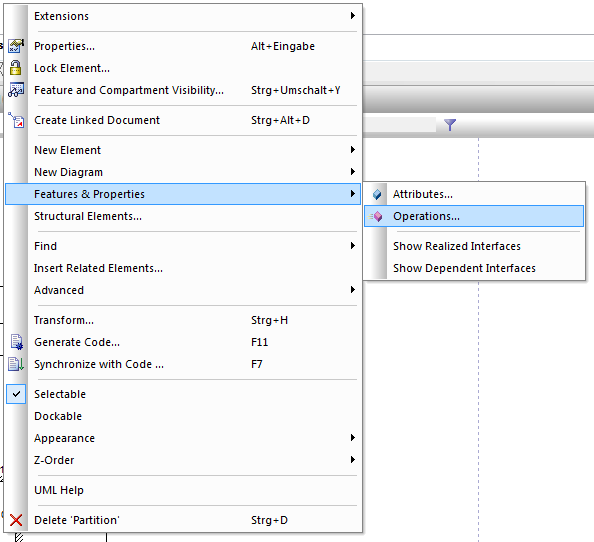
\includegraphics[width=0.7\textwidth]{ea_contextAddOperation}
	\caption{Add an operation}
	\label{fig:add_operation}
\end{figure}
\FloatBarrier

\item[$\blacktriangleright$] In the dialogue that pops-up (Fig.~\ref{fig:operation_properties}), enter \texttt{empty} as the \texttt{Name} of the operation,
leave the \texttt{Return Type} as \texttt{void}, and press \texttt{Save}.

\begin{figure}[htbp]
	\centering
  	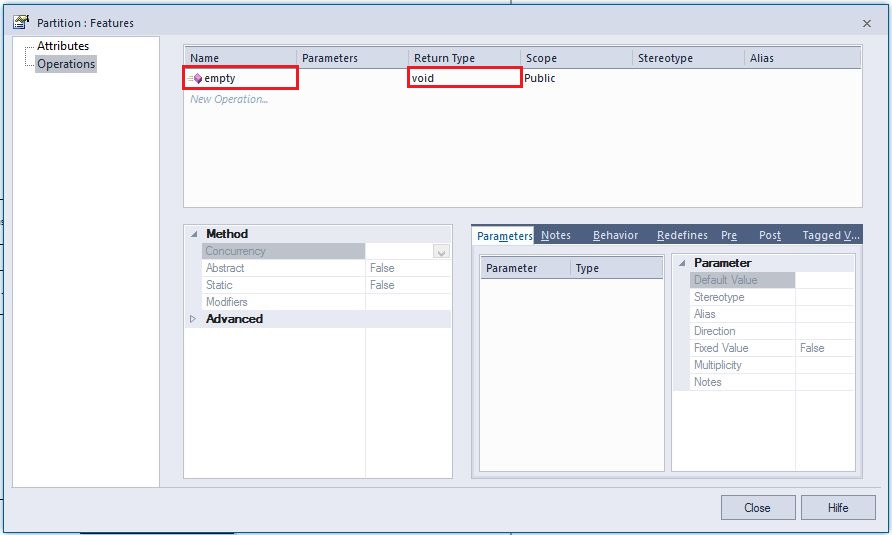
\includegraphics[width=0.5\textwidth]{ea_operationEmpty}
	\caption{Properties for operation}
	\label{fig:operation_properties}
\end{figure}
\FloatBarrier

\item[$\blacktriangleright$] In the same dialogue, press \texttt{New} to add further operations and enter the values in Fig.~\ref{fig:operation_parameters}. 
Parameters can be added by pressing \texttt{Edit}\footnote{You must save the operation before this option will become active.} and entering the name and
choosing the type of each parameter in a separate dialogue.

\begin{figure}[htbp]
	\centering
  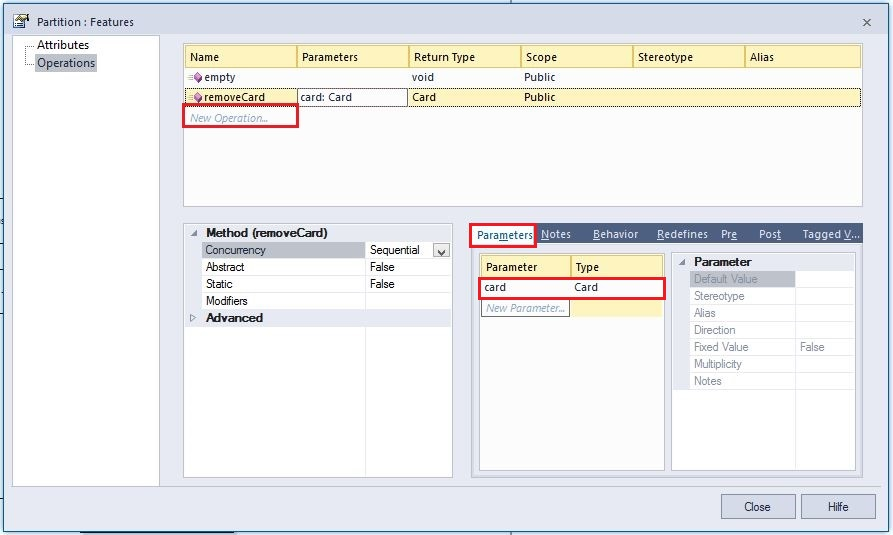
\includegraphics[width=0.9\textwidth]{ea_operationRemoveCard}
	\caption{Parameters and Return Type}
	\label{fig:operation_parameters}
\end{figure}
\FloatBarrier

\vfill
\pagebreak

\item[$\blacktriangleright$] Repeat the process for the \texttt{check} operation in Fig.~\ref{fig:operation_partition}.
Notice that the \texttt{Return Type} can be chosen via the drop-down menu for primitives (e.g. \texttt{EBoolean}), or via the `\texttt{\ldots}' button
(indicated in Fig.~\ref{fig:operation_parameters}) for types you've established in the metamodel (e.g. \texttt{Card}).

\vspace{-.5cm}
\begin{quote}
$\textbf{Please note:}$ Non-primitive types \emph{must} be chosen via the `\texttt{\ldots}' button. It allows you to browse for the corresponding elements in
your project. Just typing them won't work!
\end{quote}


\begin{figure}[htbp]
	\centering
  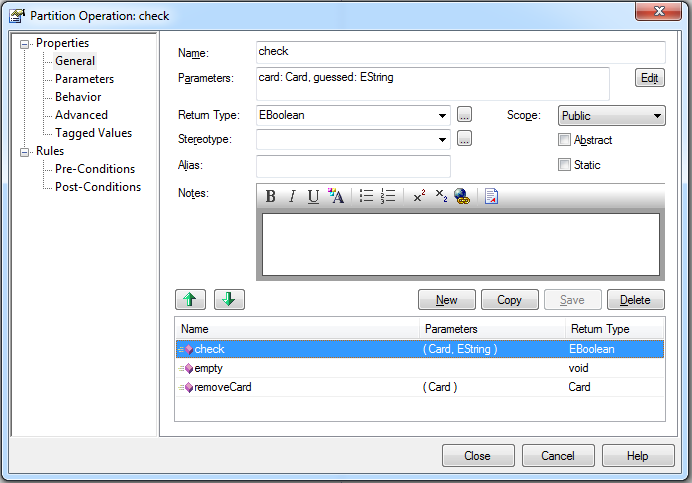
\includegraphics[width=0.9\textwidth]{ea_operationCheck}
	\caption{All operations in \texttt{Partition}}
	\label{fig:operation_partition}
\end{figure}

If you've done everything right, your dialogue should now contain three methods: \texttt{check}, \texttt{empty}, and \texttt{removeCard}, each with
corresponding parameters and return types as in Fig.~\ref{fig:operation_partition}.

Add all operations analogously for \texttt{Box} and \texttt{Card}, so that your metamodel closely resembles Fig.~\ref{fig:metamodel_complete}.

\begin{figure}[htbp]
	\centering
  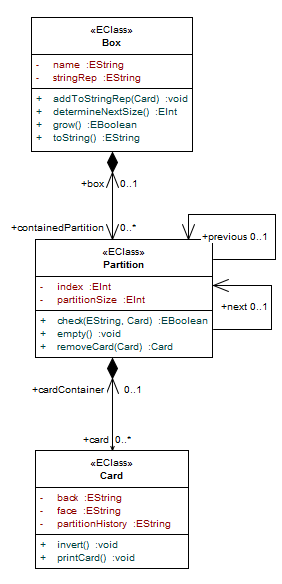
\includegraphics[width=0.7\textwidth]{ea_metamodelComplete.png}
\caption[Complete metamodel for our learning box.]{Complete metamodel for our learning box \\ \emph{\small Please note that names of parameters may not be
displayed by default in EA.}}
	\label{fig:metamodel_complete}
\end{figure}

\pagebreak

To see how this complete metamodel is represented in the textual syntax, review Fig.~\ref{fig:workspaceMethods} in \hyperlink{sec:static tex}{section 2.2}.

\item[$\blacktriangleright$] To finish, try to export the metamodel for code generation in Eclipse~\footnote{if problems occur during the following steps, we
recommend reading \texttt{Part VI: Micellaneous}. This might help you to find your mistakes}. Right-click on \texttt{LearningBoxLanguage} and choose
``Extensions/MOFLON::Ecore Addin/Export Selection to Workspace''. Then switch to your Eclipse work\-space and refresh the metamodel workingset. Alternatively,
you can activate eMoflon's add-in window by going to ``Extensions/Add-in Windows,'' and pressing \texttt{All} in the \texttt{Export} box.

\end{enumerate}

If you've done everything correctly, a new project \texttt{LearningBoxLanguage} should be created in the \texttt{Demo} working set within your eclipse
workspace. If this is not the case, please ensure that your metamodel is identical with Fig.~\ref{fig:metamodel_complete}.

If you believe everything is correct and things still don't work, feel free to contact us at \href{mailto:contact@moflon.org}{contact@moflon.org}.

If code is generated successfully, take a look at all the stuff that's been generated under \texttt{/gen}. Especially look at the the default implementation for
all methods who throw an  \texttt{OperationNotSupported} exception. We shall see later in the handbook that the Eclipse Modeling Foundation's (EMF) code
generator actually supports injecting hand-written implementations of methods into generated methods and classes. With eMoflon however, we can also model a
large part of the dynamic semantics, and only need to implement small helper methods, such as string manipulation by hand.

\fancyfoot[R]{$\triangleright$ \hyperlink{static review}{Next}}
